\section{Investigation and audit to 32 cryptocurrency exchanges}
\label{investigation}
\subsection{Security incidents and their history}
\label{subsec-incidents}
After Bitcoin was introduced in 2008, there have been many incidents happened at cryptocurrency exchange. Following are the summaries of major incidents happened in Japan.
%Table 1 shows the past major incidents which happened at cryptocurrency exchanges.
%Here, we describe the abstract of three major incidents and their source of problems.
%\begin{table}
%\begin{center}
%\caption{Major incidents at cryptocurrency exchanges}
%
%\begin{tabular}{|c|c| c | c |}\hline
%Name of Exchange & Dates & Amount of lost (at that time) & Abstract of incidents \\ \hline
%MyBitcoins & July 29, 2011 & 27,000 BTC (\$370,000) & disappear \\ \hline
%Linode & March 2012 & 46,703 BTC (\$200,000) & Web host hack\\ \hline
%Bitcoinica & March and May 2012 & 61,000 BTC &  Web host hack\\ \hline
%Bitfloor & September 2012 &24,000 BTC (\$250,000) & Server attack \\ \hline
%Mt. Gox & February 2014 & 850,000 BTC (\$473,000) & transaction malleability \\
%  &   &  &  and server hack\\ \hline
%Bitstamp & January 2015 & 19,00 BTC & Server attack \\ \hline
%Cryptsy Exchange & July 2016 &  11,325 BTC & Server attack  \\ \hline
%Bitfinex & August 2016&  119,756 BTC & Server attack  \\ \hline
%Gatecoin & 2016&  250 BTC, 185,000 ETC &  Attack on hot wallet\\ \hline
%Zaif & January 2018&  dollar &  \\ \hline
%NiceHash & December 2017 & 4,700 BTC &  Server attack \\ \hline
%CoinCheck & January 2018 & 580M dollar & Targeted attack \\ \hline
%BitHumb & June 2018 &  30M dollar  &  Server attack\\ \hline
%Monappy & September 2018 &  & Attack on hot wallet \\ \hline
%Zaif & September 2018 & 50M dollar & Attack on hot wallet \\ \hline
%\end{tabular}
%\label{table-incidents}
%\end{center}
%\end{table}

%Not all future work should be done to complete the table

\paragraph{Mt. Gox incident (2014):}

Mt. Gox was the world largest cryptocurrency exchange in 2014, which occupied about 70\% of bitcoin transaction.
The exchange did not segregate customers' assets from the exchange's asset.
The customers' assets were not recorded into Bitcoin blockchain
but recorded into some segregated ledger.
Thus, the attacker had a chance to attack the segregated
ledger instead of the attack on the blockchain and cryptographic keys itself.
The CEO of Mt. Gox claimed that the incident was caused by
transaction malleability of Bitcoin protocol.
By utilizing this vulnerability, the adversary
could convince the exchange modified transaction IDs.
This was one of factors of stealing bitcoins.% which were stored in the exchange.
Several experts pointed out that the loss was caused by this vulnerability,
but other significant factor of lost was internal malicious activities and
attack on segregated ledger from outside.



\paragraph{CoinCheck Incident (2018):}
In January 2018, CoinCheck, one of the biggest cryptocurrency exchange, but it was semi-registered to Japan Financial Service Agency (JFSA) was hacked and about 526,800,010 XEM was stolen. It was equivalent to 500M dollar. 260,000 customers of CoinCheck where victims.
This incident happened by the targeted attack as the first step. Adversary sent CoinCheck several emails to inject malware. As a result, the adversary succeeds to
intrude into the CoinCheck's network. The adversary could control computers remotely; then the adversary obtained a secret cryptographic key. After that, the adversary
sent XEM stored inside the CoinCheck's network outside within 30 minutes.
This indicates that all XEM are associated with one secret cryptographic key, and the amount of coins which each customer have is managed with a segregated ledger.
This was the same situation as the Mt. Gox incident.
The XEM stored in the hot wallet, that is the device that was connected to the internal network. Multi-signature, which is a general technique to divide signing privilege among
multiple persons, was not implemented. The main reason why CoinCheck did not implement was, the cryptographic algorithm and its parameter (elliptic curve) did not fit to
software/hardware of key management device. This implies, the kind of coin can affect the specification and operation of cryptocurrency exchange, but such
difficulties were not disclosed at that time.

\paragraph{Zaif Incident (2018):}
In September 2018, a hot wallet in Zaif was hacked and about 50M dollar equivalent Bitcoin and other cryptocurrencies were lost.
The specific problems of Zaif are it is registered cryptocurrency exchange under the current regulation. Moreover Zaif was
subject to administrative sanctions twice after the investigation described in this section. But, it did not
compliant these sanctions.

\subsection{Perspectives of investigations}
In May 2016, JFSA has amended Payment Service Act to ensure the trust of cryptocurrency users and AML/CFT, and has mandated cryptocurrency exchanges to register to JFSA and comply with legal requirements since April 2017.\footnote{JFSA has allowed companies which had already operated when the regulations was implemented to continue operation during the registration process. Thus registered exchanges and under-registration exchanges exisit as of September 2018.} In April 2017, JFSA also introduced Guidelines for administrative processes explaining how JFSA will supervise exchanges. In it, JFSA clarifies that 1) it will check each cryptocurrency if it is appropriate for exchanges to deal with from the view point of user protection and public interests, 2) it will check management's ability to ensure the operational adequacy including a) legal compliance, b) user protection, and c) risk management, and 3) foreign exchangers which provide services to people living in Japan need to register to JFSA~\cite{FSAGUIDELINE}.

After the CoinCheck incident, JFSA conducted monitoring on all the 32 companies and the on-site inspections of 7 registered and all the 16 under-registeration exchanges to check if they comply with the regulation. In so doing, JFSA clarifies that it reviews the business practices, the risks and compliance management, as well as the internal audit and corporate culture/governance, especially focusing on the perspectives including 1) the practice of assessment on the risk characteristics of the cryptocurrency a company deals with, 2) adequacy of risk management, 3) practice on anti-money laundering and anti-illicit activities, and 4) Practice on segregation of customers' assets

On the basis of the findings from the on-site inspection, JFSA issued business improvement orders and business suspension orders to those companies with problems. It also turned down the registration request from one company. Receiving these orders, 12 under-registration companies gave up registration.

\subsection{Results of investigation and audit}
On August 10, 2018, JFSA published an interim report of the results of the on-site inspection and the monitoring with the aim of helping cryptocurrency exchanges to improve their business practices and regulatory compliance~\cite{FSAREPORT}. In section 2 of the report, JFSA shows numbers related to exchanges\footnote{Fig 1 to 3 and Fig 4 to 6 in the following shown in Page 4 and Page 5 of the JFSA's report respectively.}. Fig 1 shows the number of total assets of 13 registered and four under-registration exchanges in the last business year and Fig 2 shows the amount in the latest business year.
Fig 3 shows the change in the amount of total asset in one business year, which growth reaches on average 553\%. The report explains the massive increase of the total asset was caused by the hike in the exchange rate of the cryptocurrency against fiat currency since fall in 2017. Fig 4 shows the number of employees of all exchanges and Fig 5 shows customers' assets they manage. Based on these numbers, the report calculated the amount of customers' assets that one employee manages shown in Fig 6. JFSA point out by citing this number that very few people manage the huge amount of customers' assets; on average, one person manages \$30 million. %To give a sense of scale, this number is larger than \$16 million, which is the amount of deposit that one employee manages at MUFG, the largest Japanese financial group\cite{MUFG}.
JFSA explains that the establishment of the internal management was too slow to keep up with the rapid business expansion and management lacks awareness of the risks associated with the custody service managing the huge amount of customers' assets.

JFSA shows findings within the business practices, the risk and compliance management, and the internal audit and corporate culture/governance as summarized in the following.

\begin{center}
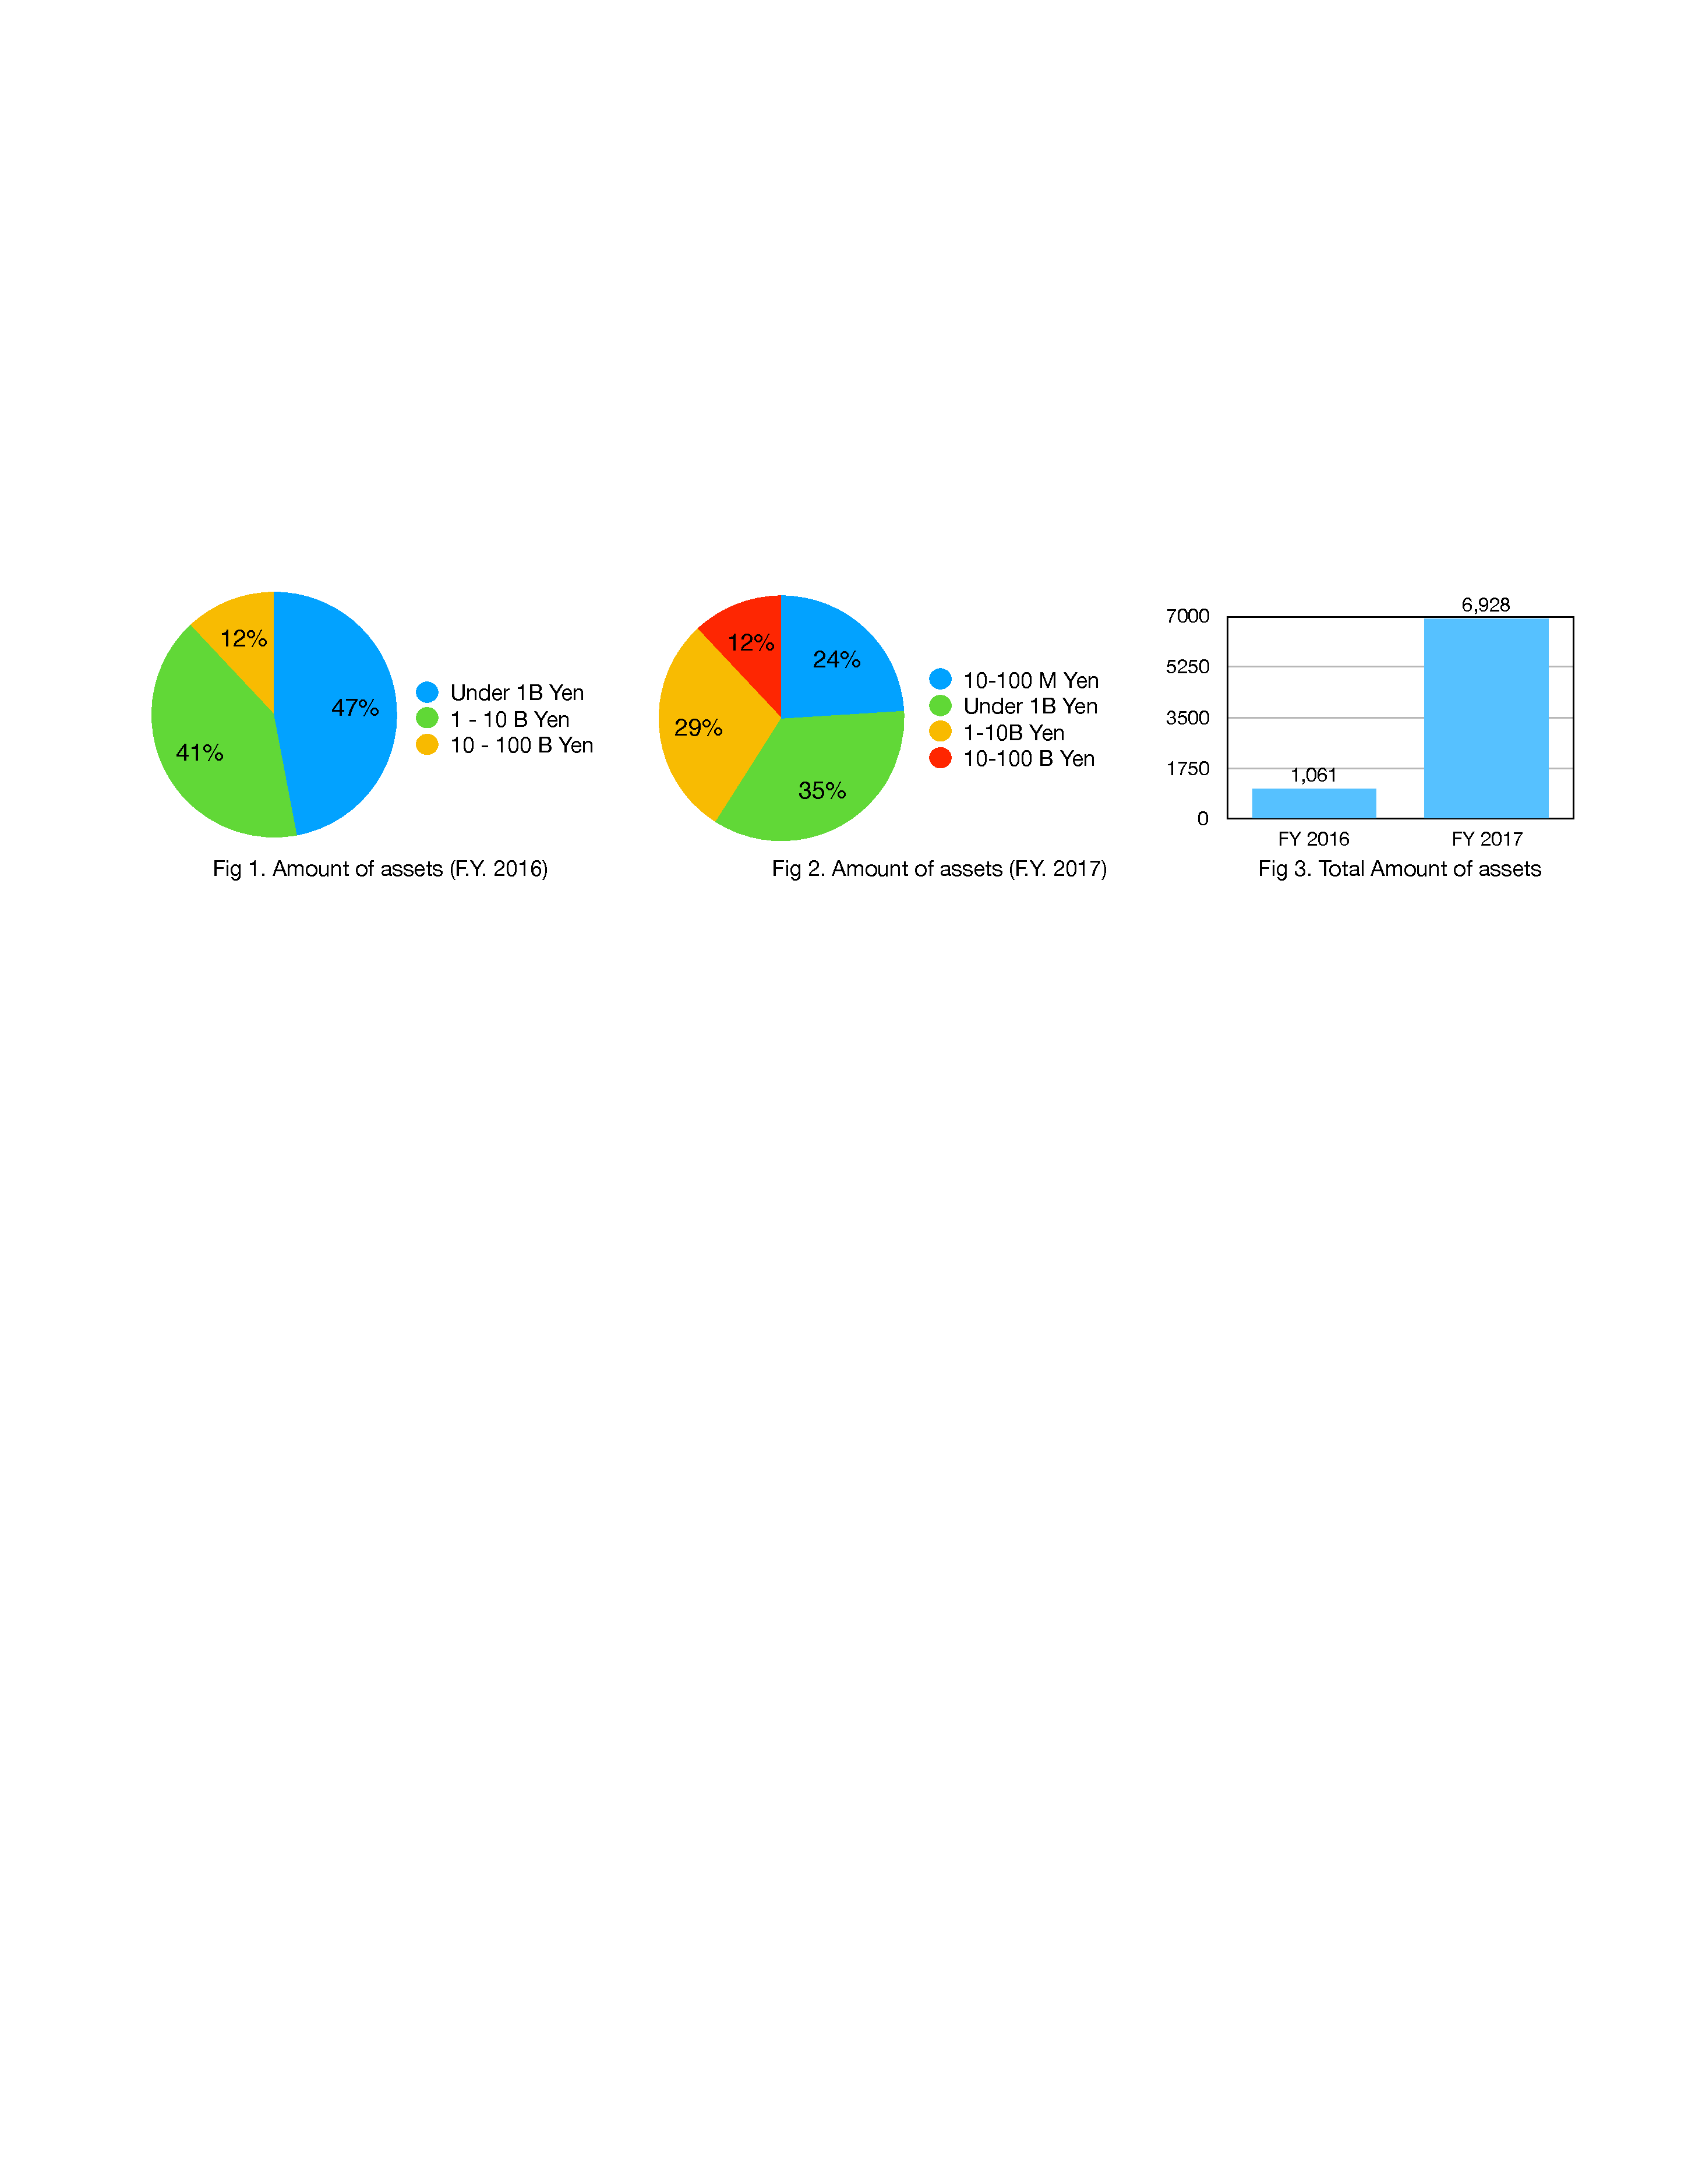
\includegraphics[width=9cm,pagebox=cropbox,clip]{fig1.pdf}
\end{center}

\begin{center}
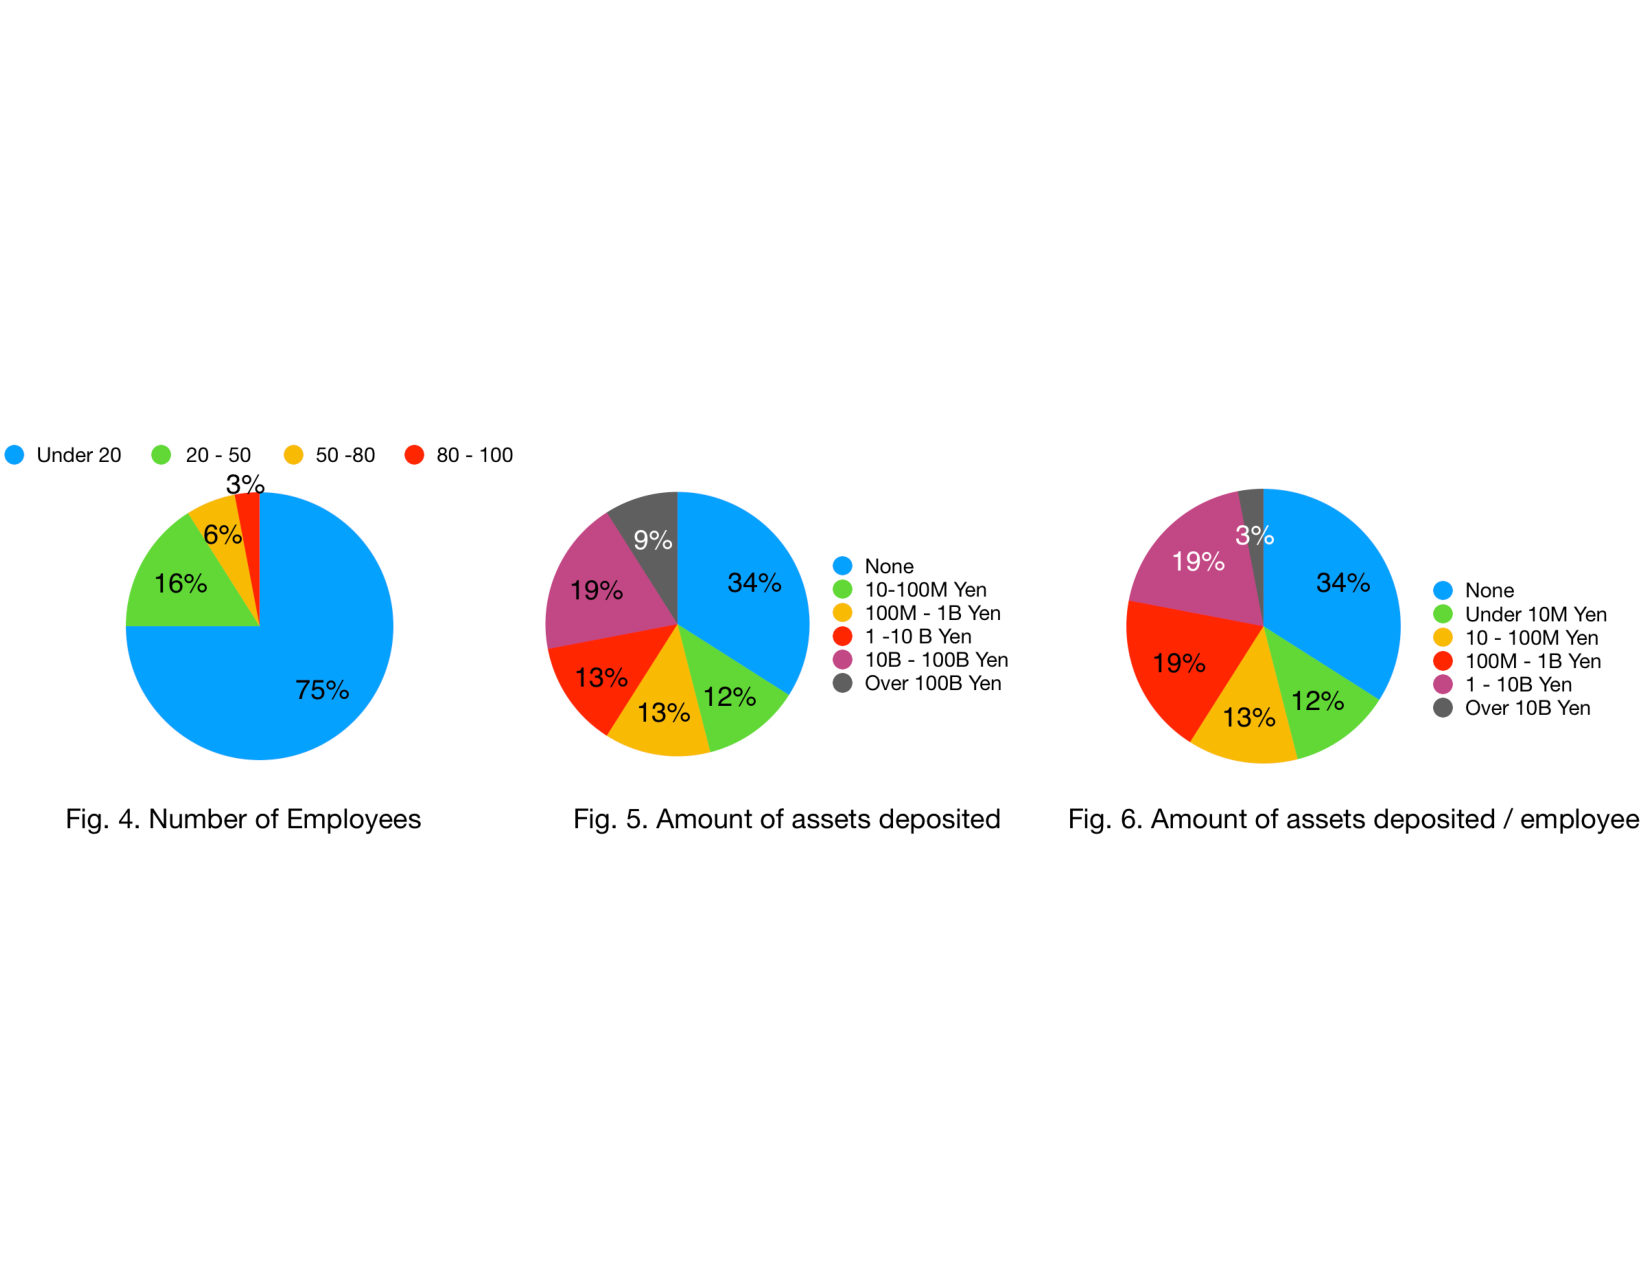
\includegraphics[width=9cm,pagebox=cropbox,clip]{fig2.pdf}
\end{center}

\subsubsection{Frontline: The business practices}
The report points out the issues around 1) selection process of cryptocurrency to deals with, 2) inappropriate distribution of cryptocurrency and 3) advertisement.
More concretely, the report explains that many\footnote{"Many" in this section means JFSA found similar issues in 8 or more exchanges.} exchanges lack business practices to assess risks associated with each cryptocurrency while they focus only on customer convenience and the profitability. And several\footnote{"Several" in this section means JFSA found similar issues in 2 to 7 exchanges.} exchanges lack internal rules that define investment limits and criteria for solicitation and transaction based on the `'principle of suitability' concerning customers' characteristics. The report even points out a case of price manipulation. There also found cases where advertisements of exchanges could mislead users.
%there is a case where an exchange does not have the internal review process of the contents of the advertisement. With regard to the advertisement itself, an exchange used TV advertisement on which famous celebrity calls the name of the certain cryptocurrency to encourage customers to buy it while explains risks only in few seconds. In another case, an advertisement shows a particular discount period and investment profitability that customers cannot verify.

\subsubsection{Second line: The risk and compliance management}
The report points out the issues around 1) AML/CFT, 2) segregation of customers' assets, 3) system risk management, 4) customer protection, 5) third party delegation.

For AML/CFT, several exchanges lack enough experts who can provide appropriate advice to frontline staff regarding risk managment. Thus many exchanges fail to comply with the regulation that requires multi-layer countermeasures for AML/CFT such as the establishment of internal guidelines, conducting customer due diligence, and monitoring of suspicious activities. The report shows a case where an exchange allows an organized crime group member to continue transaction for a while after the exchange realized that the customer is a member the group.
%In addition, there are issues around practices as well. For example, many exchanges fail to comply with the regulation that requires them to confirm customers' characteristics and purpose of the transaction as well as conduct pre-examination to exclude transactions with the anti-social group. There are cases of lack of appropriate guidelines regarding checking process of impersonation, and an exchange lacks monitoring process and system to detect suspicious activities.

For segregation of customers' assets, JFSA explains that several exchanges manage cryptocurrency in the hot (online) wallet, fail to reconcile on the daily basis between account balance within their server and that on the blockchain, and lack an ex-post verification process of reconciliation. Several exchanges also combine customers' assets and their own assets in order to keep the amount on the blockchain larger than the account balance within internal server. There is a case where an exchange even does not segregate customers' assets at all for some cryptocurrency. Yet another exchange, even when it recognizes that the account balance of internal server becomes below the balance on the blockchain, neither appropriately identify the cause nor address it. The report also points out the issues related to management of fiat currency in a similar manner. Furthermore, JFSA found that several exchanges fail to follow regulatory requirements on bookkeeping and an exchange even diverts money to other purposes.
%In addition, JFSA points out the issue around management of fiat currency. For example, several exchanges fail to reconcile between bank account balance for customers' assets and account balance on their own server.  Yet another exchange fails to find out the cause of the frequent incident that the customers' bank account balance becomes below the balance on their own server. Furthermore, JFSA found issues around bookkeeping. For example, several exchanges create general ledger only and fail to keep books on daily transactions, the ledger of their own account, and the ledger of customers' account, all of which are required by regulation.

For systemic risk management, JFSA shows that many exchanges lack human resources and training to manage the information system and fail to establish a contingency plan based on the risk scenario on cyber attacks. An exchange even issues new crypto assets without conducting a security evaluation of the underlining technology. JFSA also points out problems on authority management and countermeasures toward system troubles. For instance, within several exchanges, the same person develops and operates the system, and an exchange also fails to impose appropriate restrictions on holders of administrative IDs. Lack of record keeping and efforts to address the root cause of system troubles are also pointed out. In addition, lack of awareness of system limitation caused over capacityof of trading volume in an exchange.

For customer protection, the report mentions problems related to crypto assets issuance. There are several cases found in individual exchanges such as %lack of explanation about the financial situation and business model of the issuing exchange to customers,
failure to keep promise that the money raised is invested in new businesses, lack of clear understanding on accounting practices for cryptocurrency issuance, failure to disclose any unfair treatment including the huge discounts for insiders or realized differences between reality and the white paper. %and the huge bonus to management of the exchange for sale of the cryptocurrency.
JFSA also found issues that several exchanges fail to establish customer information management guidelines, %fail to conduct the training program on these matters, fail
lack access control on customer information and fail to address customer complaimnts in an appropriate way%, and allow anyone in the company and third-party contractor to access to it or even bring out from the company
.
%Several exchanges fail to either keep records of the customer complains or improve the business practice based on the complaints. They just ignore them or randomly address them case by case basis.
The report also shows examples where exchanges fail to conduct the assessment on volatility and trading volume of the cryptocurrency to decide loss-cut or set leverage limitation of margin trading.

For third-party outsourcing, the report explains several individual cases. For example, an exchange neither conduct the assessment of third-party contractor nor establish a formal outsourcing contract. %For another example, an exchange does not manage third-party contractor and fails to check the situation of outsourcing from the third party contractor. Another exchange does not request a third-party system developer to address issues related to system troubles.
Another exchange using cloud service fails to establish an outsourcing contract with its provider because of the lack of awareness that the cloud server is the third party to manage.

\subsubsection{Third line: The internal audit}
The report reveals that there are no internal audit or the internal audit is not based on the risk assessment within several exchanges. In many exchanges, there are not enough experts in internal audit implementation regarding AML/CFT and system risk management. For example, many exchanges fail to conduct the internal audit% or establish the plan for internal audit
because only one person who has another position is assigned to the position in charge of internal audit. %For other examples, several exchanges fail to conduct it based on the risk assessment or to conduct the audit on the third party contractor.
Furthermore, in an exchange, a person who is in charge of internal audit reports no problem even though the person, in fact, did not verify it.

\subsubsection{Corporate culture and governance}
The reports point out that exchanges prioritize profit making and lack culture of compliance and customer protection and internal management. For example. JFSA found that many exchanges fail to hire enough staff and improve IT system to support the expansion of the business. There is a case where management meeting focuses solely on expansion and advertisement but not on internal management. In an exchange, major shareholders and the management are not separated and management prioritizes profit of these shareholders.

Even though exchanges are in essence financial institutions, engineers who lack expertise in financial business manage the company. From the first point, many exchanges even lack awareness that they are financial institution dealing with huge amount of customers' assets% and fail to discuss how to mitigate risks associated with their business in the board meeting. The report also mentions that many exchanges fail to disclose their business and financial situation to customers in an easy-to-understand manner.

The weak management by the company's Board of Directors is also an issue. It is often the case that the CEO has too much power and the Board and internal audit fail to check the management. For example, several exchanges fail to keep the record of the Board meeting and the Board members are not well informed to play an appropriate role. For another example, the Board members fail to check if the money raised by token issuance is used as promised or check if the external auditor has enough knowledge and experience to conduct the appropriate audit.
